\documentclass[12pt,oneside]{book}
%\geometry{bindingoffset=0cm}
%\documentclass[prl,aps, 12pt]{revtex4}
%\documentclass[1pt]{revtex4}%{article} \usepackage{amssymb}
\providecommand{\ei}[1]{\color{red}[#1]\color{black}}

\renewcommand{\thesection}{\arabic{section}}
\renewcommand{\thesubsection}{\arabic{subsection}}

\pagestyle{plain} \textwidth=16.5cm \oddsidemargin=0cm \textheight=23cm
\topmargin=-1.25cm

\renewcommand{\baselinestretch}{1.0}


\usepackage{mdframed}
\usepackage[T1]{fontenc}
\usepackage{graphicx}
\usepackage{amssymb}
\usepackage{amsmath}
\newcommand\numberthis{\addtocounter{equation}{1}\tag{\theequation}}
%\usepackage[fleqn]%{amsmath}
%\usepackage{caption}
%\usepackage{subcaption}
\usepackage{color}
%\usepackage{xcolor}
\usepackage[dvipsnames]{xcolor}
\usepackage{slantsc}
\usepackage{float}
\graphicspath{{./FIG_FINALI/}}
\usepackage{bbold}
\usepackage[caption=false]{subfig}
\usepackage{array}
\usepackage{lipsum}
%\floatstyle{boxed}
%\restylefloat{figure}
\usepackage{braket}
%\usepackage{breqn}
\usepackage{scrextend}
\usepackage{changepage}
\setlength\multlinegap{0pt}
\captionsetup[subfigure]{labelformat=empty}
\usepackage{hyperref}
\hypersetup{backref,pdfpagemode=FullScreen,colorlinks=true,allcolors=blue}
\usepackage{leftidx}
\newcommand{\rededit}[1]{\textcolor{red}{#1}}
\newcommand{\greenedit}[1]{\textcolor{green}{#1}}
\newcommand{\blueedit}[1]{\textcolor{blue}{#1}}

\usepackage{mathtools}
\DeclarePairedDelimiter\brac{\langle}{\rvert}
\DeclarePairedDelimiter\cket{\lvert}{\rangle}

\DeclareMathOperator*{\argmin}{arg\,min}
\title{Quantum Computing Primer for Electronic-Structure}
\author{Subhayan Roychoudhury\\ The Molecular Foundry\\ Lawrence Berkeley National Laboratory}
\date{}
%\affil{LBNL}


\begin{document}

\maketitle

\subsection*{Electronic Structure Theory and the Problem of Scaling}

Any general single-particle state $\ket{\phi}$ can be expressed with respect to position vectors (eigenvectors of the position operator) $\ket{\mathbf{r}}$ as
\begin{align*}
    \ket{\phi} &{}= \int d \mathbf{r} \ket{\mathbf{r}}\braket{\mathbf{r}|\phi}\\
    &{} = \int d\mathbf{r} \phi(\mathbf{r})\ket{\mathbf{r}}, \numberthis
\end{align*}
where we have defined
\begin{align}
    \phi(\mathbf{r})= \braket{\mathbf{r}|\phi}.
\end{align}

For the sake of computational feasibility, we need to work with a discrete set of points within a real space grid. Then, we need to replace the integral with a sum as

\begin{align}\label{OneP_Expansion}
    \ket{\phi} = \sum_{i=1}^m \phi_i \ket{\mathbf{r}_i},
\end{align}
where $m$ denotes the total number of grid points, $\ket{\mathbf{r}_i}$ is the position-vector associated with the $i$-th grid point, and 
\begin{align}
    \phi_i=\braket{\mathbf{r}_i|\phi}.
\end{align}

Eq.~\ref{OneP_Expansion} shows that, in this representation, our basis set $\{\ket{\mathbf{r}_1}, \ket{\mathbf{r}_2},\hdots, \ket{\mathbf{r}_m}\}$ has $m$ number of basis vectors. What happens if, instead of a single particle, we need to describe a two-particle state within the same grid? Now our basis set becomes something like
\begin{align*}
    \{\ket{\mathbf{r}_1\mathbf{r}_1}, \ket{\mathbf{r}_1\mathbf{r}_2} , \hdots , \ket{\mathbf{r}_1\mathbf{r}_m}, \ket{\mathbf{r}_2\mathbf{r}_1} , \ket{\mathbf{r}_2\mathbf{r}_2}, \hdots , \ket{\mathbf{r}_2\mathbf{r}_m}, \hdots , \ket{\mathbf{r}_m\mathbf{r}_1}, \ket{\mathbf{r}_m\mathbf{r}_2}, \hdots , \ket{\mathbf{r}_m\mathbf{r}_m}\},
\end{align*}
where 
\begin{align*}
\ket{\mathbf{r}_i \mathbf{r}_j} = \ket{\mathbf{r}_i}\otimes\ket{\mathbf{r}_j}.
\end{align*}

Thus, we now have $m^2$ basis vectors in our set. Generalizing to an $N$-particle system, we will need $m^N$ number of basis vectors, implying that the generic state resides in a $m^N$ dimensional space. This is an example of exponential scaling with respect to the number of particles.

For the purpose of describing a many-electron system, a couple of additional points need to be taken into account.
\begin{enumerate}
    \item Electrons have an additional \textit{spin} degree of freedom, which, for a single particle, requires two basis vectors. Denoting such a basis-set by $\{\ket{\uparrow},\ket{\downarrow}\}$, the single-electron basis set must now be modified to 
    \begin{align*}
        \{\ket{\mathbf{r}_1}\otimes\ket{\uparrow}, \ket{\mathbf{r}_1}\otimes\ket{\downarrow}, \ket{\mathbf{r}_2}\otimes\ket{\uparrow}, \ket{\mathbf{r}_2}\otimes\ket{\downarrow},\hdots, \ket{\mathbf{r}_m}\otimes\ket{\uparrow}, \ket{\mathbf{r}_m}\otimes\ket{\downarrow}\}.
    \end{align*}
    This has $M = 2m$ number of basis vectors.  We shall call them spin-orbitals in the position basis. By extension, for $N$-particles, we will need $(M)^N$ basis vectors. For $\alpha \in \{\uparrow,\downarrow\}$, we will use the notation $\ket{\mathbf{r}_i^\alpha}$ to denote $\ket{\mathbf{r}_i}\otimes\ket{\alpha}$.
    \item Electrons are indistinguishable particles with wavefunctions that are antisymmetric with respect to an exchange of any two electrons. This implies, for example, that
    \begin{align}
        \ket{\mathbf{r}_i^\alpha\mathbf{r}_j^\beta} = -\ket{\mathbf{r}_j^\beta\mathbf{r}_i^\alpha},
    \end{align}
    and therefore, we do not need to consider them separately when we construct our basis set. We can, in fact, combine them into the so-called Slater determinants.

    This also implies that
\begin{align}
\ket{\mathbf{r}_i^\alpha\mathbf{r}_i^\alpha}=-\ket{\mathbf{r}_i^\alpha\mathbf{r}_i^\alpha}=\ket{0}.
\end{align}

\end{enumerate}

Therefore, from our basis set, we can discard any vector in which the same spin-orbital is occupied by multiple electrons. These considerations will reduce the number of vectors required for our $N$-particle basis set. Any basis vector that we need to include in our new basis set can now be uniquely defined by specifying which spin-orbitals are occupied and which ones are empty (since no spin-orbital can have multiple occupancy and since, thanks to indistinguishability, we do not care which electron is in which orbital). Thus, each basis vector corresponds to choosing $N$ number of occupied spin-orbitals from a total number of $M$. Therefore, instead of $(M)^N$, now the number of basis-vectors in our set should be $_{M}C_N$ (the binomial coefficient \textit{$M$ choose $N$}). Let us find out what these basis vectors should look like.

If there are $M$ number of spin-orbitals, then any such basis vector (analogous to a Slater determinant) can be expressed as
\begin{align}\label{SD_OccupationRepresentation}
    \ket{\mathrm{B}}=\ket{j_{M-1}j_{M-2}\hdots j_1 j_0},
\end{align}
where, for any $i=0,\hdots,M-1$, the value of $j_i$ can be either 0 or 1. In this convention, $j_i=0$ and $j_i=1$ will indicate, respectively, that the $(i+1)$-th spin-orbital is empty and occupied. Since each spin-orbital can only have two possible occupancies (0 or 1), the number of possible Slater determinants can not exceed $2^M$. However, if the total number of electrons is known to be $N$, then we know that every Slater determinant must have exactly $N$ number of occupied orbitals. Then, as mentioned earlier, the possible number of Slater determinants boils down to $_MC_N$, which, for any $N$, can never exceed $2^M$.

Let us take a concrete example. If there are 2 electrons in our system (like in a hydrogen molecule), then, the representation of an arbitrary electronic state on a $10 \times 10 \times 10$ real space grid will require $_{2000}C_2$ i.e, 1999000 basis vectors. Consequently, we need to store 1999000 number of coefficients if we want to store this state (written as a linear combination of the basis vectors) on a computer. Assuming each coefficient requires a byte of storage, we will need slightly less than 2 MB. 

If there are 42 electrons in our system (like in a benzene molecule), then the number of basis vectors is $_{2000}C_{42}$. This has the order of $10^{87}$. Therefore, the number of bytes required to store all the coefficients will exceed the estimated number of atoms in the universe!

One may say ``well, I blame our choice of spin-orbitals. Why don't we use a set of atom-centred basis-functions instead?''. Indeed, this reduces the memory-requirement by quite a lot. For example, if we use the $\textit{minimal}$ atom-centred basis orbitals, then, for benzene we need 36 spatial functions. Each hydrogen atom will have a single $1s$-like function while each carbon atom will have 5 functions (one each for $1s$ , $2s$ , $2p_x$, $2p_y$ and $2p_z$). Therefore, we need a total of $M = 36 \times 2 =72$ spin-orbitals. Now, instead of $\sim 10^{87}$, we will need $_{72}C_{42} \approx 1.6 \times 10^{20}$ bytes to store the generic state. However, for pentacene ($\mathrm{C}_{22}\mathrm{H}_{14}$), the number of minimal spin-orbitals will be $M = 3080$ and consequently the storage requirement will be $_{3080}C_{146} \approx 5.5 \times 10^{253}$.

This points to the fact that a wise choice of spin-orbitals can mitigate the problem only to a certain extent and only for very small systems. The real issue is not the choice affecting $M$, but the expression governing the scaling, i.e., $_MC_N$.

On a conventional computer, the increment in memory is linear with the increment in the number of storage units. If you double the number of bits, you get twice as much memory. However, the scaling of $_{M}C_N$  with respect to $N$ or $M$ (unless $N=1$ or $N\approx M$) is substantially higher. Thus, in practice, if we really want to store all the necessary coefficients on a memory-device, we need a device whose capacity (with respect to the number of storage units) scales \textit{at least} as quickly as $_{M}C_N$. This is exactly where a quantum computer can help.


%Now, the state of a qubit, the unit of information of a quantum computer, resides in a 2-dimensional Hilbert space and thereby, requires two basis vectors for its description. Let us choose a set of orthonormal basis vectors in this Hilbert space and denote them by $\ket{0}$ and $\ket{1}$. Naturally, an arbitrary state of $n$ qubits is expressible as a linear-combination of $2^n$ basis vectors. Thus, the dimension of the relevant Hilbert space, and consequently the storage capacity increases exponentially with the number of qubits.


Let us find out how we can represent a general many-electron state, written as a linear combination of $_MC_N$ basis vectors (the form of a generic basis vector was shown in Eq.~\ref{SD_OccupationRepresentation}), with the help of a quantum computer? %Note that every basis 


%We can now easily represent the aforementioned Slater determinant with qubits. In a quantum-representation using qubits, we can adapt a convention whereby, the $i$-th qubit being in state $\ket{1}$ will indicate that the $(i+1)$-th spin-orbital is occupied while the state $\ket{0}$ for the qubit will indicate an unoccupied $(i+1)$-th spin-orbital. 


    
    %It suffices to combine them into a single basis-vector $\ket{\mathbf{r}_i^\alpha\mathbf{r}_j^\beta} - \ket{\mathbf{r}_j^\beta\mathbf{r}_i^\alpha}$.
    
    %A two-electron state $\ket{\Phi} = C_1 \ket{\mathbf{r}_i^\alpha\mathbf{r}_j^\beta} + C_2 \ket{\mathbf{r}_j^\beta\mathbf{r}_i^\alpha} + \hdots$ can be written simply as $\ket{\Phi} = (C_1-C_2) \ket{\mathbf{r}_i^\alpha\mathbf{r}_j^\beta}+\hdots$

\subsection*{The Qubit}

For a quantum computer, the unit of information is a qubit. The state of a single qubit resides in a 2-dimensional vector space. Naturally, any basis-set of this space contains two basis vectors. Let us choose a set where the two orthogonal basis vectors are denoted by $\ket{0}$ and $\ket{1}$. Thus, any general vector 
\begin{align}\label{Eq1}
    \ket{a}=a_0\ket{0}+a_1\ket{1}
\end{align}
can be expressed in matrix-form as $\begin{pmatrix}
        a_0\\
        a_1
    \end{pmatrix}$.

Naturally, the basis-vectors $\ket{0}$ and $\ket{1}$ themselves will be written as
$\begin{pmatrix}
        1\\
        0
    \end{pmatrix}$ and $\begin{pmatrix}
        0\\
        1
    \end{pmatrix}$, respectively.

A tensor product of $\ket{a}$ (Eq.~\ref{Eq1}) and $\ket{b}=b_0\ket{0}+b_1\ket{1}$ is then given by

\begin{align}\label{Eq2}
    \ket{ab}=\ket{a}\otimes\ket{b}=a_0b_0 \ket{0}\otimes\ket{0} + a_0b_1 \ket{0}\otimes\ket{1} +a_1b_0 \ket{1}\otimes\ket{0} + a_1b_1\ket{1}\otimes\ket{1}.
\end{align}
$\ket{ab}$ resides in a 4-dimensional space which is the tensor-product space of the two aforementioned vector spaces (i.e., one which hosts $\ket{a}$ and one which hosts $\ket{b}$). If we choose to use $\{\ket{0}\otimes\ket{0} , \ket{0}\otimes\ket{1}, \ket{1}\otimes\ket{0}, \ket{1}\otimes\ket{1}\}$ as the basis-set of this space, then, in matrix form, the vector $\ket{ab}$ can be expressed as $\begin{pmatrix}
    a_0b_0\\
    a_0b_1\\
    a_1b_0\\
    a_1b_1
\end{pmatrix}.$

For example, the two-qubit state $\ket{01}$ can be written as $\begin{pmatrix}
    0\\
    1\\
    0\\
    0
\end{pmatrix}$

This notion can be generalized to more than 2 qubits in a straightforward manner. Continuing the convention introduced in Eq.~\ref{Eq1} and~\ref{Eq2}, for the $2^n$ dimensional vector space of $n$ qubits, we will choose the basis set
\begin{align*}
\{\ket{0,0,\hdots,0,0} , \ket{0,0,\hdots,0,1} , \ket{0,0,\hdots,1,0}, \ket{0,0,\hdots,1,1},\hdots ,\ket{1,1,\hdots,1,1} \}.
\end{align*}
Each basis vector contains $n$ terms, each of which can be either 0 or 1. The basis vectors are ordered in such a way that, for each vector, the rightmost term changes between every consecutive vector. The next (to the left) term remains unchanged for two consecutive vectors and then changes. Continuing in this fashion, it is easy to see that the leftmost term remains unchanged at 0 for the first $2^{n-1}$ basis vectors and then stays fixed at 1 for the rest of the vectors. Such a basis set will be referred to as a computational basis set for $n$ qubits.

\subsection*{Many-electron States : a Qubit-based Representation}

From the discussion presented above, we can see that any computational basis-vector of $M$ qubits can be written as

\begin{align}\label{M_qubit_basis}
    \ket{B} = \ket{q_{M-1}q_{M-2}\hdots q_1 q_0},
\end{align}
where, for any $i=0,\hdots,M-1$, the value of $q_i$ can be either 0 or 1. It is easy to notice the resemblance between Eq.~\ref{M_qubit_basis}, i.e., a basis-vector of the $M$-qubit Hilbert space and Eq.~\ref{SD_OccupationRepresentation}, a basis-vector for a many-electron system with $M$ spin-orbitals. Therefore, in order to represent an arbitrary many-electron state using qubits, we can adopt a convention whereby, the $i$-th qubit being in state $\ket{1}$ will indicate that the $(i+1)$-th spin-orbital is occupied while the state $\ket{0}$ for the same qubit will indicate an unoccupied $(i+1)$-th spin-orbital. Then, any general many-electron state of any number ($<M$) of electrons, expressible as a linear-combination of Slater determinants composed of $M$ spin-orbitals (see Eq.~\ref{SD_OccupationRepresentation}), can be represented by some general $M$-qubit state constructed as a linear-combination of the computational basis-vectors (Eq.~\ref{M_qubit_basis}). Thus, in contrast with a conventional computer which requires $_MC_N$ bytes to store an $N$-electron state (as discussed earlier, this number is $\sim 10^{20}$ for a benzene molecule even if we use a minimal basis set), a quantum computer can store the same state with $M$ qubits (i.e., 72 qubits for the benzene example).

However, being able to merely represent a many-electrons states with the help of qubits is not enough. Typically, we would be interested in \textit{solving} an electronic-structure problem such as finding a specific eigenstate of a given operator, finding the evolution of a given state with time, etc. To this end, we will typically need the ability to apply operators (for example, the Hamiltonian or the time-evolution operator) on the many-electron states. In the context of quantum computation, this, naturally, means that we need operators for the qubit space. 

\subsection*{Quantum Gates}

In the context of quantum-circuits, an $n$-qubit operator is essentially an $n$-qubit gate that changes an $n$-qubit quantum state from some initial state $\ket{I}$ to some final state $\ket{F}$.

Naturally, an operator in an $N$-dimensional space can be uniquely defined by specifying its actions on the basis functions (which are $N$ in number) of any basis set of that space. Working with the computational basis set introduced earlier, the Hadamard gate $\hat{H}$ for the 1-qubit space can be defined as
\begin{align*}\label{Hadamard}
    \hat{H}\ket{0} &{}= \frac{1}{\sqrt{2}}\left(\ket{0}+\ket{1}\right) = \ket{+}\\
    \hat{H}\ket{1} &{}= \frac{1}{\sqrt{2}}\left(\ket{0}-\ket{1}\right) = \ket{-}\numberthis
\end{align*}
The orthonormality of $\{\ket{0},\ket{1}\}$ implies that
\begin{align*}
    \braket{0|\hat{H}|0}=\frac{1}{\sqrt{2}}, \hspace{1cm} \braket{0|\hat{H}|1}=\frac{1}{\sqrt{2}}, \hspace{1cm} \braket{1|\hat{H}|0}=\frac{1}{\sqrt{2}}, \hspace{1cm}
    \braket{1|\hat{H}|1}=-\frac{1}{\sqrt{2}}.
\end{align*}
Therefore, with respect to the computational basis set, $\hat{H}$ can be written in matrix form as
\begin{align}
    \frac{1}{\sqrt{2}}\begin{pmatrix}
        1 & 1\\ 1 & -1
    \end{pmatrix}
\end{align}
Another 1-qubit gate is the Pauli gate $\hat{X}$ whose operations are given by
\begin{align*}
    \hat{X}\ket{0} = \ket{1} \hspace{0.5cm} \mathrm{and} \hspace{0.5cm} \hat{X}\ket{1}=\ket{0},
\end{align*}
indicating a matrix representation of $\begin{pmatrix}
    0 & 1\\ 1 & 0
\end{pmatrix}$.
A tensor-product of $n$ number of single-qubit operators (each operator associated with a 2-dimensional vector space) is an operator acting on $n$ qubits (associated with a $2^n$ dimensional vector space). With this in mind, let us construct a simple 2-qubit operator from $\hat{X}$ and $\hat{H}$ such that its operation on the state $\ket{ab}$ (see Eq.~\ref{Eq2}) follows
\begin{align}
\hat{XH}\left(\ket{ab}\right)&{}=\left(\hat{X}\ket{a}\right)\otimes\left(\hat{H}\ket{b}\right)\\
&{}=\left(a_0\ket{1}+a_1\ket{0}\right) \otimes \frac{1}{\sqrt{2}} \left(b_0\ket{+}+b_1\ket{-}\right)
\end{align}
Note that the final state after operation of $\hat{XH}$ can be written as a simple tensor-product of two single-qubit states. Thus, after the operation, the second qubit will be in the state $\left(a_0\ket{1}+a_1\ket{0}\right)$ and the first qubit will be in the state $\left(b_0\ket{+}+b_1\ket{-}\right)$ with a normalization factor of $\frac{1}{\sqrt{2}}$. Thus, the final state is \textbf{not entangled}. This is not surprising, given that the 2-qubit operator $\hat{XH}$ itself is a simple tensor-product of 2 single-qubit operators.

Let us see an example where this is no longer true. 

A controlled gate acts on a 2-qubit state in such a way that, if the control qubit is in state $\ket{0}$, then it performs an identity operation ($\hat{I}$) on the target qubit. However, if the control qubit is in state $\ket{1}$, then the controlled gate will perform a predefined operation on the target qubit. A controlled NOT (CNOT) gate, for which the predefined operation is a Pauli $\hat{X}$ operation, is a well-known example. Denoting the left and the right qubit respectively as the control and the target qubit, we have

\begin{align*}
    \hat{\mathrm{CNOT}}\ket{00} &{}= \ket{0} \otimes \left(\hat{I}\ket{0}\right)= \ket{00}\\
    \hat{\mathrm{CNOT}}\ket{01} &{}= \ket{0} \otimes \left(\hat{I}\ket{1}\right) = \ket{01}\\
    \hat{\mathrm{CNOT}}\ket{10} &{}= \ket{1} \otimes \left(\hat{X}\ket{0}\right) = \ket{11}\\
    \hat{\mathrm{CNOT}}\ket{11} &{}=  \ket{1} \otimes \left(\hat{X}\ket{1}\right) = \ket{10},\\
\end{align*}
which indicates a matrix form of $\begin{pmatrix}
    1 & 0 & 0 & 0\\ 0 & 1 & 0 & 0\\0 & 0 & 0 & 1\\ 0 & 0 & 1 & 0
\end{pmatrix}$.

Acting on the 2-qubit state $\ket{+0}$, this will produce
\begin{align*}
    \hat{\mathrm{CNOT}} \ket{+0} &{}= \frac{1}{\sqrt{2}} \hat{\mathrm{CNOT}} \ket{00} + \frac{1}{\sqrt{2}} \hat{\mathrm{CNOT}} \ket{10}\\
    &{}= \frac{1}{\sqrt{2}} \left(\ket{00}+\ket{11}\right).
\end{align*}
This can not be written as a tensor product of 2 single-qubit states. If we measure the state of the first qubit (in this context, when I say ``\textit{measure the state}'' of a qubit, what I mean is ``\textit{measure the observable corresponding to the operator $\hat{Z}$, for which the eigenvectors are $\ket{0}$ and $\ket{1}$}'') and get, for example, the eigenvalue corresponding to $\ket{1}$, then we know immediately that the entire 2-qubit system must have collapsed to the state $\ket{11}$. Therefore, if we measure the state of the second qubit immediately, we are guaranteed to get $\ket{1}$. Thus, in the state $\hat{\mathrm{CNOT}}\ket{+0}$, the two qubits are entangled! Under these circumstances, there is no such thing as ``state of the first qubit'' or ``state of the second qubit''.

The controlled rotation CROT gate is another example of a contolled gate. This gate performs a rotation operation $\hat{U}_\theta$ by a predefined angle $\theta$ such that
\begin{align}\label{kickback1}   \hat{U}_\theta\ket{\psi}=e^{i\theta}\ket{\psi}
\end{align}
on the target qubit, if the control qubit is $\ket{1}$.

Let us operate this on the 2-qubit state $$\frac{1}{\sqrt{2}}\left(\ket{0}+\ket{1}\right)\otimes\ket{1} = \frac{1}{\sqrt{2}}\left(\ket{01}+\ket{11}\right)$$. This should produce
\begin{align*}\label{kickback2}
    \frac{1}{\sqrt{2}}\left(\ket{01}+\exp^{i\theta}\ket{11}\right) = \frac{1}{\sqrt{2}} \left(\ket{0}+\exp^{i\theta}\ket{1}\right)\otimes\ket{1}.\numberthis
\end{align*}
Interestingly, the operation has altered the state of the control qubit from $\frac{1}{\sqrt{2}}\left(\ket{0}+\ket{1}\right)$ to $\frac{1}{\sqrt{2}}\left(\ket{0}+\exp^{i\theta}\ket{1}\right)$, leaving the state of the target qubit intact at $\ket{1}$. In other words, a rotation was essentially applied to the control qubit, even though the rotation operator $\hat{U}_\theta$ acted only on the target qubit. The result of the phase-rotation of the target qubit is effectively kicked back onto the control qubit. This effect is called \textbf{phase kickback}.
Now we will use this effect to construct a quantum circuit that can solve a crucial problem, namely that of finding the discrete Fourier transform.

A periodic function $f(x)$ with a period of $l$ can be written as a linear combination of its Fourier components as
\begin{align}\label{Fourier1}
    f(x)=\frac{1}{\sqrt{l}}\sum_{k=-\infty}^{+\infty} \tilde{f}(k) e^{-2\pi i\frac{kx}{l}},
\end{align}
where $\tilde{f}(k)$ is given by
\begin{align}
    \tilde{f}(k) = \frac{1}{\sqrt{l}}\int_0^l f(x) e^{2\pi i \frac{xk}{l}} dx.
\end{align}
Discretizing the problem, the discreet Fourier transform of a sequence of $N$ complex numbers $\{f(0),f(1),\hdots,f(N-1)\}$ (if we assume that the sequence repeats itself after an interval of $N$, we can compare the elements of this sequence with the values of $f(x)$ from Eq.~\ref{Fourier1} at a discrete set of points) can be defined as
\begin{align}\label{Fourier_tilde_expansion}
    \tilde{f}(k) = \frac{1}{\sqrt{N}} \sum_{j=0}^{N-1} f(j) e^{2\pi i \frac{jk}{N}}.
\end{align}
To avoid any possible confusion, it is important to mention that the sign of the exponent is a matter of convention. In fact, typically, for discrete Fourier transform, a negative exponent is used. However, in keeping with the standard convention of quantum Fourier transform (QFT), we are keeping it positive.

We would want the QFT operator $\hat{U}_{\rm{QFT}}$ to transform a vector with expansion-coefficients $\{f(0),f(1),\hdots,f(N-1)\}$ into a vector with coefficients $\{\tilde{f}(0),\tilde{f}(1),\hdots,\tilde{f}(N-1)\}$. In mathematical terms:

\begin{align}\label{QFT_1}
    \hat{U}_{\rm{QFT}} \left(\sum_{k=0}^{N-1} f(k)\ket{k}\right) = \sum_{k=0}^{N-1}\tilde{f}(k)\ket{k},
\end{align}

where $\ket{k}$ is the $k$-th vectors of the computational basis set. Notably, the basis set contains $N$ number of basis vectors. Therefore, this $N$-dimensional vector space is associated with $n=log_2(N)$ qubits. Taking inner product of both sides of Eq.~\ref{QFT_1} with $\bra{j}$ and summing over $j$,

\begin{align*}
    \sum_{j=0}^{N-1}\sum_{k=0}^{N-1} f(k)\braket{j|\hat{U}_\mathrm{QFT}|k} &{}=  \sum_{j=0}^{N-1}\sum_{k=0}^{N-1} \tilde{f}(k)\delta_{j,k}\\
    &{}=\sum_{j=0}^{N-1}\tilde{f}(j)\\
    &{}=\frac{1}{\sqrt{N}} \sum_{j=0}^{N-1}\left(\sum_{k=0}^{N-1} f(k) e^{2\pi i \frac{kj}{N}}\right)
\end{align*}
where, in the third equality we have used the expansion of $\tilde{f}(j)$ in accordance with Eq.~\ref{Fourier_tilde_expansion}. The above equation implies
\begin{align*}
    \braket{j|\hat{U}_\mathrm{QFT}|k} &{}= \frac{1}{\sqrt{N}} e^{2\pi i \frac{kj}{N}},
\end{align*}
i.e.,
\begin{align*}
    \hat{U}_\mathrm{QFT} = \frac{1}{\sqrt{N}} \sum_{l=0}^{N-1}\sum_{k=0}^{N-1} e^{2\pi i \frac{kl}{N}} \ket{k}\bra{l}
\end{align*}
Now, we will try to express
\begin{align}\label{QFT_2}
    \hat{U}_\mathrm{QFT}\ket{j} &{}=\frac{1}{\sqrt{N}} \sum_{k=0}^{N-1}e^{2\pi ij\frac{k}{N}}\ket{k}.
\end{align}
as a tensor-product of $n$ number of single-qubit states. At this point, it is necessary to express the integer $k$ in terms of its binary representation. If $k$ can be written in binary form as $$k_{n-1}k_{n-2}\hdots k_0 \hspace{2cm} \textrm{ where } k_i \in \{0,1\} \forall i=0,\hdots,n-1,$$
where $k_0$ is the least significant bit, then
\begin{align*}
    k=k_{n-1}2^{n-1}+k_{n-2}2^{n-2}+\hdots+k_02^0.
\end{align*}
Therefore,
\begin{align*}\label{EqBinaryExpansion}
    \frac{k}{N}=\frac{k}{2^n} = \sum_{t=0}^{n-1} \frac{k_t}{2^{n-t}}.\numberthis
\end{align*}
Plugging this expression back into Eq.~\ref{QFT_2}, the following equation is obtained:
\begin{align*}\label{QFT_main}
    \hat{U}_\mathrm{QFT}\ket{j} &{}= \frac{1}{\sqrt{N}} \sum_{k=0}^{N-1} e^{2\pi ij \left( \sum_{t=0}^{n-1} \frac{k_t}{2^{n-t}} \right)}\ket{k}\\
    &{} = \frac{1}{\sqrt{N}} \sum_{k=0}^{N-1} \left(\prod_{t=0}^{n-1} e^{2\pi ij \frac{k_t}{2^{n-t}}}\right) \ket{k}\\
    &{} = \frac{1}{\sqrt{N}} \sum_{k_{n-1}=0}^1 \hdots \sum_{k_1=0}^1\sum_{k_0=0}^1 \left( e^{2\pi ij \frac{k_{n-1}}{2}} \ket{k_{n-1}}\right)\otimes \hdots \otimes \left( e^{2\pi ij \frac{k_1}{2^{n-1}}} \ket{k_1}\right) \otimes \left( e^{2\pi ij \frac{k_0}{2^n}} \ket{k_0}\right)\\
    &{} = \frac{1}{\sqrt{N}} \left(\sum_{k_{n-1}=0}^1 \left( e^{2\pi ij \frac{k_{n-1}}{2}} \ket{k_{n-1}}\right) \right) \otimes \hdots \otimes \left(\sum_{k_1=0}^1 e^{2\pi ij \frac{k_1}{2^{n-1}}} \ket{k_1}\right) \otimes \left(\sum_{k_0=0}^1 e^{2\pi ij \frac{k_0}{2^n}} \ket{k_0}\right)\\
    &{} = \frac{1}{\sqrt{N}} \left(\ket{0} + e^{\frac{2\pi ij}{2}}\ket{1}\right) \otimes \hdots \otimes \left( \ket{0} + e^{\frac{2\pi i j}{2^{n-1}}}\ket{1} \right)\otimes \left(\ket{0}+e^{\frac{2\pi i j}{2^n}}\ket{1}\right)\numberthis
\end{align*}
where, in the third line, we have expressed the $k$-th computational basis vectors as a tensor product of single-qubit basis vectors $$\ket{k}=\ket{k_{n-1}}\otimes\hdots\otimes\ket{k_0}.$$ This lets us convert the sum over $k$, i.e., over all computational basis functions of the $2^n$ dimensional space (as shown in the second line) into individual sums over each constituent qubit (as shown in the third line):
\begin{align*}
    \sum_{k=0}^{N-1} \rightarrow \sum_{k_{n-1}=0}^1 \hdots \sum_{k_0=0}^1
\end{align*}

Now we are ready to show that, if the basis-vector $\ket{j}$ is fed into the input of the quantum circuit shown in Fig.~\ref{QFT_circuit} in such a way that the bottommost (topmost) qubit corresponds to the least (most) significant bit, then the transformed state shown in the RHS of Eq.~\ref{QFT_main} is obtained as the output. This circuit contains the Hadamard gate $\hat{H}$ (see Eq.~\ref{Hadamard}) and the controlled rotation $\hat{\mathrm{CROT}}$ gate which we redefine (in a slightly different way) below. If the control qubit is $\ket{0}$, the $\hat{\mathrm{CROT}}_k$ gate performs, as expected, an identity operation on the target qubit. On the other hand, if the control qubit is $\ket{1}$, then a $\hat{R}_k$ operation is performed on the target qubit $\ket{T}$ such that
\begin{align*}
\hat{R}_k\ket{T}=e^{\frac{2\pi i T}{2^k}}\ket{T}
\end{align*}

In our circuit diagram, the two-qubit operation $\hat{\mathrm{CROT}}_k$ is shown by the construction of Fig.~\ref{Fig.CROT_k} where the black dot indicates the operation on the control qubit and the boxed $\hat{R}_k$ indicates the (conditional) rotation operation on the target qubit.

\begin{figure}
    \centering
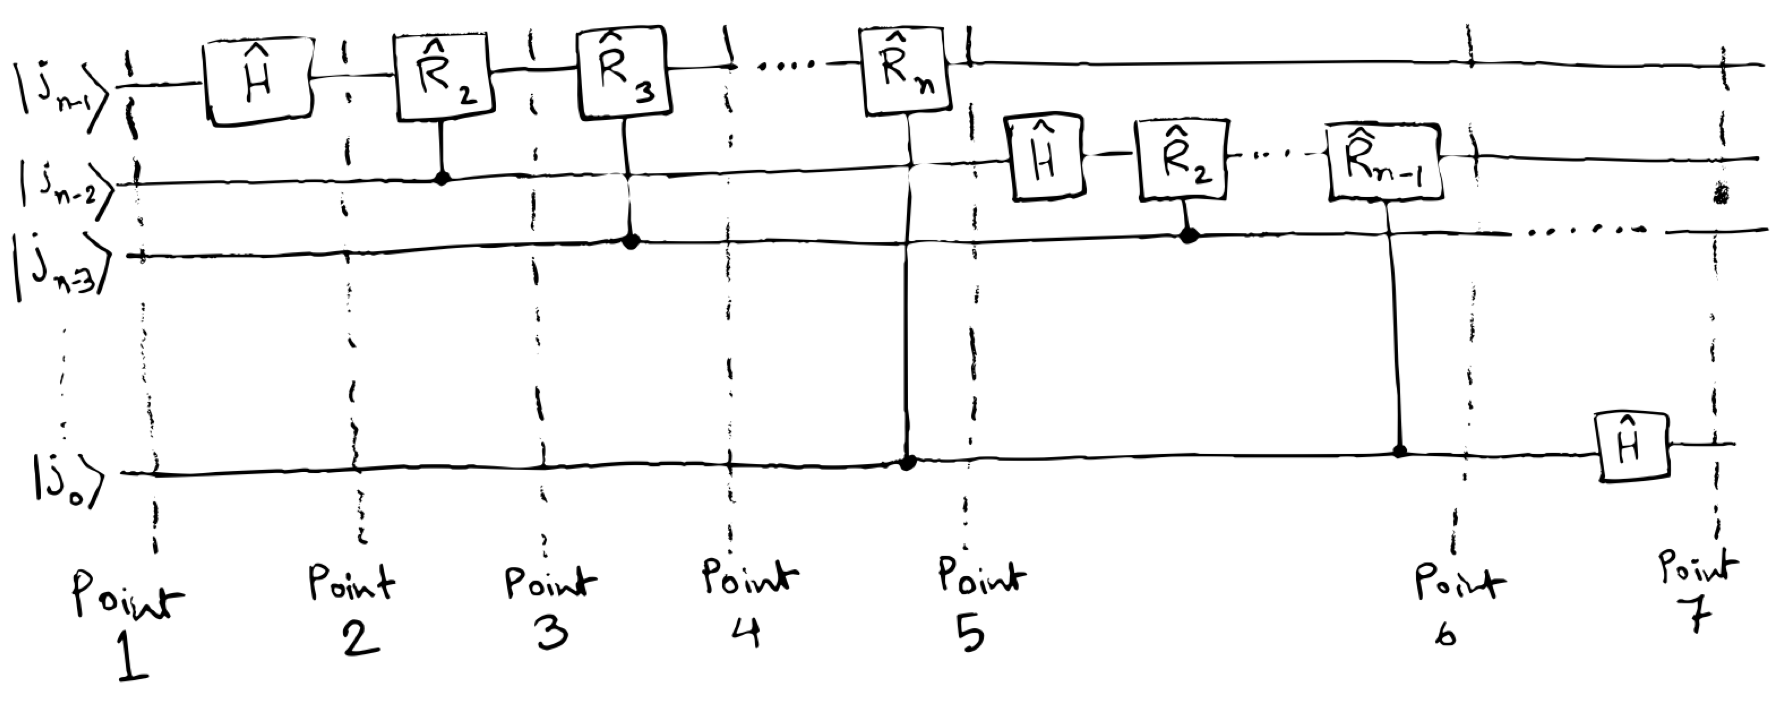
\includegraphics[width=0.99\textwidth]{QFT_schematic.png}
    \caption{Circuit for performing quantum Fourier transform}
    \label{QFT_circuit}
\end{figure}

Now let us take a close look at Fig.~\ref{QFT_circuit}.

\begin{figure}
    \centering   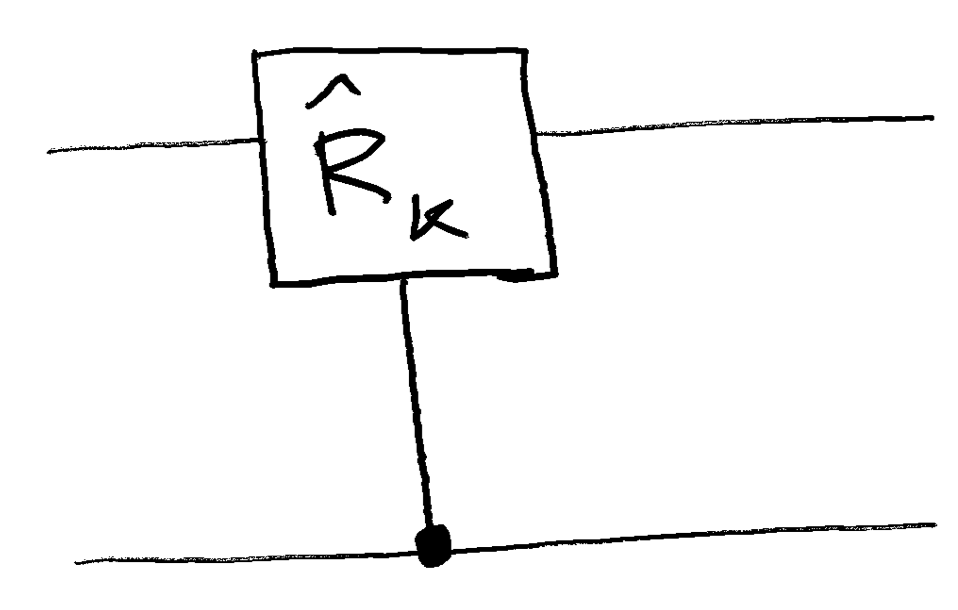
\includegraphics[width=0.5\textwidth]{CROT_gate.png}
    \caption{The $\hat{\mathrm{CROT}_k}$ gate}
    \label{Fig.CROT_k}
\end{figure}

\begin{enumerate}
    \item At the input point (point 1), we have the state $$\ket{j_{n-1} j_{n-2}\hdots j_1 j_0}.$$
    Remember that this is the $j$-th computational basis vector and so the qubits represent the integer $j$ in binary form.
    \item Then a Hadamard gate acts on the topmost qubit, leaving the others intact. Consequently, at point 2 we have 
    \begin{align*}
        \left(\hat{H}\ket{j_{n-1}}\right)\otimes\ket{j_{n-2}\hdots j_1 j_0} = \frac{1}{\sqrt{2}}\left(\ket{0}+e^{\frac{2\pi i j_{n-1}}{2}}\ket{1}\right)\otimes \ket{j_{n-2}\hdots j_1 j_0}
    \end{align*}
    \item Next a controlled rotation $\hat{\mathrm{CROT}}_2$ is applied on the topmost target qubit with the qubit below it serving as the control qubit. The resulting state at point 3 is
    \begin{align*}
\hat{\mathrm{CROT}}_2\left(\ket{0}\otimes\ket{j_{n-2}}+e^{\pi i j_{n-1}}\ket{1}\otimes\ket{j_{n-2}}\right)\otimes \frac{1}{\sqrt{2}}\ket{j_{n-3}\hdots j_0}
    \end{align*}
    Note from the circuit diagram that, of the two qubits involved in the $\hat{R}_2$ operation, the state $\ket{j_{n-2}}$ acts as the control qubit. Note that $$\hat{R}_2\ket{0}=e^{\frac{2\pi i.0}{2^2}}\ket{0}=\ket{0},$$
    and therefore, 
    $$\hat{\mathrm{CROT}}_2\left(\ket{0}\otimes\ket{j_{n-2}}\right) = \ket{0}\otimes\ket{j_{n-2}}.$$
    What about $\hat{\mathrm{CROT}}_2 \ket{1}\otimes\ket{j_{n-2}}$?
    If $\ket{j_{n-2}}=\ket{0}$, then obviously the state remains intact:
    \begin{align*}
        \hat{\mathrm{CROT}}_2 \ket{1}\otimes\ket{j_{n-2}} &{}= \ket{1}\otimes\ket{j_{n-2}}\\
        &{} = e^{\frac{2\pi ij_{n-2}}{2^2}}\ket{1}\otimes\ket{j_{n-2}}
    \end{align*}
    
    If $\ket{j_{n-2}}=\ket{1}$ then
    \begin{align*}
        \hat{\mathrm{CROT}}_2 \ket{1}\otimes\ket{j_{n-2}} &{} = e^{\frac{2\pi i.1}{2^2}}\ket{1}\otimes\ket{j_{n-2}}\\
        &{} = e^{\frac{2\pi ij_{n-2}}{2^2}}\ket{1}\otimes\ket{j_{n-2}}
    \end{align*}
    
    Then the state at point 3 simplifies to
    \begin{align*}
       &{} \left(\ket{0}\otimes\ket{j_{n-2}}+e^{\pi i j_{n-1}}e^{\frac{2\pi i j_{n-2}}{2^2}}\ket{1}\otimes\ket{j_{n-2}}\right) \otimes \frac{1}{\sqrt{2}}\ket{j_{n-3}\hdots j_0}\\
       &{} = \left(\ket{0}+e^{2\pi i \left(\frac{j_{n-1}}{2^1}+\frac{j_{n-2}}{2^2}\right)}\ket{1}\right) \otimes \frac{1}{\sqrt{2}}\ket{j_{n-2}\hdots j_0}\\
    \end{align*}
    \item In an identical way, it follows that the state at point 4 is
    \begin{align*}
         \left(\ket{0}+e^{2\pi i \left(\frac{j_{n-1}}{2^1}+\frac{j_{n-2}}{2^2}+\frac{j_{n-3}}{2^3}\right)}\ket{1}\right) \otimes \frac{1}{\sqrt{2}}\ket{j_{n-2}\hdots j_0}
    \end{align*}
    \item In this way, the topmost qubits picks up a phase with every controlled rotation upto point 5. At this point the state becomes
    \begin{align*}
        &{}\left(\ket{0}+e^{2\pi i \sum_{t=0}^{n-1}\frac{j_t}{2^{n-t}}}\ket{1}\right) \otimes \frac{1}{\sqrt{2}}\ket{j_{n-2}\hdots j_0}\\
        &{}=\left(\ket{0}+e^{2\pi i\frac{j}{2^n}}\ket{1}\right) \otimes \frac{1}{\sqrt{2}}\ket{j_{n-2}\hdots j_0}
    \end{align*}
    where we have used Eq.~\ref{EqBinaryExpansion}.
    From now on, the topmost qubit remains unchanged.
    \item In a similar manner, beyond point 6, the next qubit (the one below the topmost qubit) remains unchanged. At this point, the state of the system is
    \begin{align*}
        \left(\ket{0}+e^{2\pi i\frac{j}{2^n}}\ket{1}\right) \otimes \left(\ket{0}+e^{2\pi i\frac{j}{2^{n-1}}}\ket{1}\right) \otimes \frac{1}{\sqrt{2^2}}\ket{j_{n-2}\hdots j_0}
    \end{align*}
\item Finally, at point 7, the state is
\begin{align*}
    \frac{1}{\sqrt{2^n}} \left(\ket{0}+e^{2\pi i\frac{j}{2^n}}\ket{1}\right) \otimes \left(\ket{0}+e^{2\pi i\frac{j}{2^{n-1}}}\ket{1}\right) \otimes \hdots \otimes \left(\ket{0} + e^{\frac{2\pi ij}{2}}\ket{1}\right)
\end{align*}
\item If we could record this output in the reverse order (i.e., topmost qubit first), we would obtain the expression on the RHS of Eq.~\ref{QFT_main}.
\end{enumerate}

What we have done here is to show that if the input of the circuit (Fig.~\ref{QFT_circuit}) is the computational basis vector $\ket{j}$, then the output, in the reverse order of qubits, is the state on the RHS of Eq.~\ref{QFT_main}. If this state is written as a linear combination of the computational basis vectors, then one recovers the expression on the RHS of Eq.~\ref{QFT_2}. As expected, the coefficients of expansion denote the discreet Fourier transform of a sequence of numbers $\{\delta_{1,j}, \delta_{2,j}, \hdots, \delta_{j,j},\hdots,\delta_{N,j}\}$ (which are essentially the coefficients of expansion of $\ket{j}$ with respect to the computational basis).

How can we go about finding the QFT of a generic state $\ket{X}=\sum_{j=0}^{2^n-1} f(j)\ket{j}$? 

Naturally,
\begin{align*}\label{QFT_generic}
    \hat{U}_{\mathrm{QFT}}\ket{X} &{}= \sum_{j=0}^{2^n-1} f(j) \hat{U}_{\mathrm{QFT}} \ket{j}\\
    &{}=\frac{1}{\sqrt{N}} \sum_{j=0}^{N-1} f(j) \left(\sum_{k=0}^{N-1}e^{2\pi ij\frac{k}{N}}\ket{k}\right)\\
    &{} = \frac{1}{\sqrt{N}} \sum_{k=0}^{N-1} \left( \sum_{j=0}^{N-1} f(j) e^{2\pi ij\frac{k}{N}}\right) \ket{k}\\
    &{} = \frac{1}{\sqrt{N}} \sum_{k=0}^{N-1} \tilde{f}(k)\ket{k},\numberthis
\end{align*}
where, in the second line we have used Eq.~\ref{QFT_2} and in the fourth line we have used Eq.~\ref{Fourier_tilde_expansion}. Therefore, as expected from the linearity of the QFT operator, if we use a generic state $\ket{X}$ as the input for the circuit of Fig.~\ref{QFT_circuit}, the output, read in the reverse order, will be its QFT.

If we want the discrete Fourier transform of the sequence $\{f(0),f(1),\hdots,f(N-1)\}$, then, first of all, we have to prepare the input state as $\sum_{j=0}^{N-1}f(j)\ket{j}$ (unfortunately, this is not always possible in an efficient manner). Then we will feed this into the circuit of Fig.~\ref{QFT_circuit} and measure the output. If we repeat the entire process for say, $\tau$ number of times, then at different iterations, the measurement will collapse the final state to different vectors of the computational basis.
%
If the number of collapses to the state $\ket{k}$, recorded in the reverse order, is $\tau_k$, then we can conclude that $|\tilde{f}(k)|=\left(\frac{\tau_k}{\tau}\right)^{0.5}$.

Notably, excluding the number of operations required for the preparation of the initial state, the number of operations required in the circuit (Fig.~\ref{QFT_circuit}) is $n + (n-1) + \hdots + 1=\frac{n(n+1)}{2}$, which scales polynomially with respect to the number of qubits.

\subsection*{Quantum Phase Estimation}

Now we will tackle a problem with potentially paramount importance in electronic structure theory. Given an operator in the qubit space, how can we find its eigenvalues and eigenstates\footnote{We have already seen how to represent a many-electron state in the qubit-space. Later we will discuss how to represent an electronic operator in the qubit space}.
%
To this end, let us start with a simpler problem.
%
Given an operator and one of its eigenstates in the qubit space, how can we find the corresponding eigenvalue?
%
Let the operator and the state be $\hat{O}$ and $\ket{\Psi}$, respectively, such that 
\begin{align}
    \hat{O}\ket{\Psi}=\phi\ket{\Psi},
\end{align}
$\phi$ being the eigenvalue. Naturally, we can construct an operator $\hat{U}=e^{2\pi i \hat{O}}$ such that
\begin{align}
    \hat{U}\ket{\Psi}=e^{2\pi i \phi}\ket{\Psi}.
\end{align}
From our earlier example of phase-kickback (see Eq.~\ref{kickback1} and~\ref{kickback2}), it is easy to see that if $\hat{U}$ is operated as a controlled gate on the target state $\ket{\Psi}$, with the control qubit being in state $\frac{1}{\sqrt{2}}(\ket{0}+\ket{1})$, then the control qubit will be rotated by an angle dependent on the eigenvalue of $\ket{\Psi}$. This is the property we will exploit for our goal.

In particular, the operation of Controlled-$\hat{U}^{2^t}$ on $\frac{1}{\sqrt{2}}(\ket{0}+\ket{1}) \otimes \ket{\Psi}$, with the left (right) state denoting the control (target) state will produce
\begin{align*}\label{representativeCROT}
    C-\hat{U}^{2^t} \left[\frac{1}{\sqrt{2}}(\ket{0}+\ket{1}) \otimes \ket{\Psi}\right] &{} = \frac{1}{\sqrt{2}}\left(\ket{0}+\left(e^{2\pi i \phi}\right)^{2^t}\ket{1}\right) \otimes \ket{\Psi}\\
    &{} = \frac{1}{\sqrt{2}}\left(\ket{0}+\left(e^{2^t . 2\pi i \phi}\right)\ket{1}\right) \otimes \ket{\Psi}\numberthis
\end{align*}

\begin{figure}
    \centering
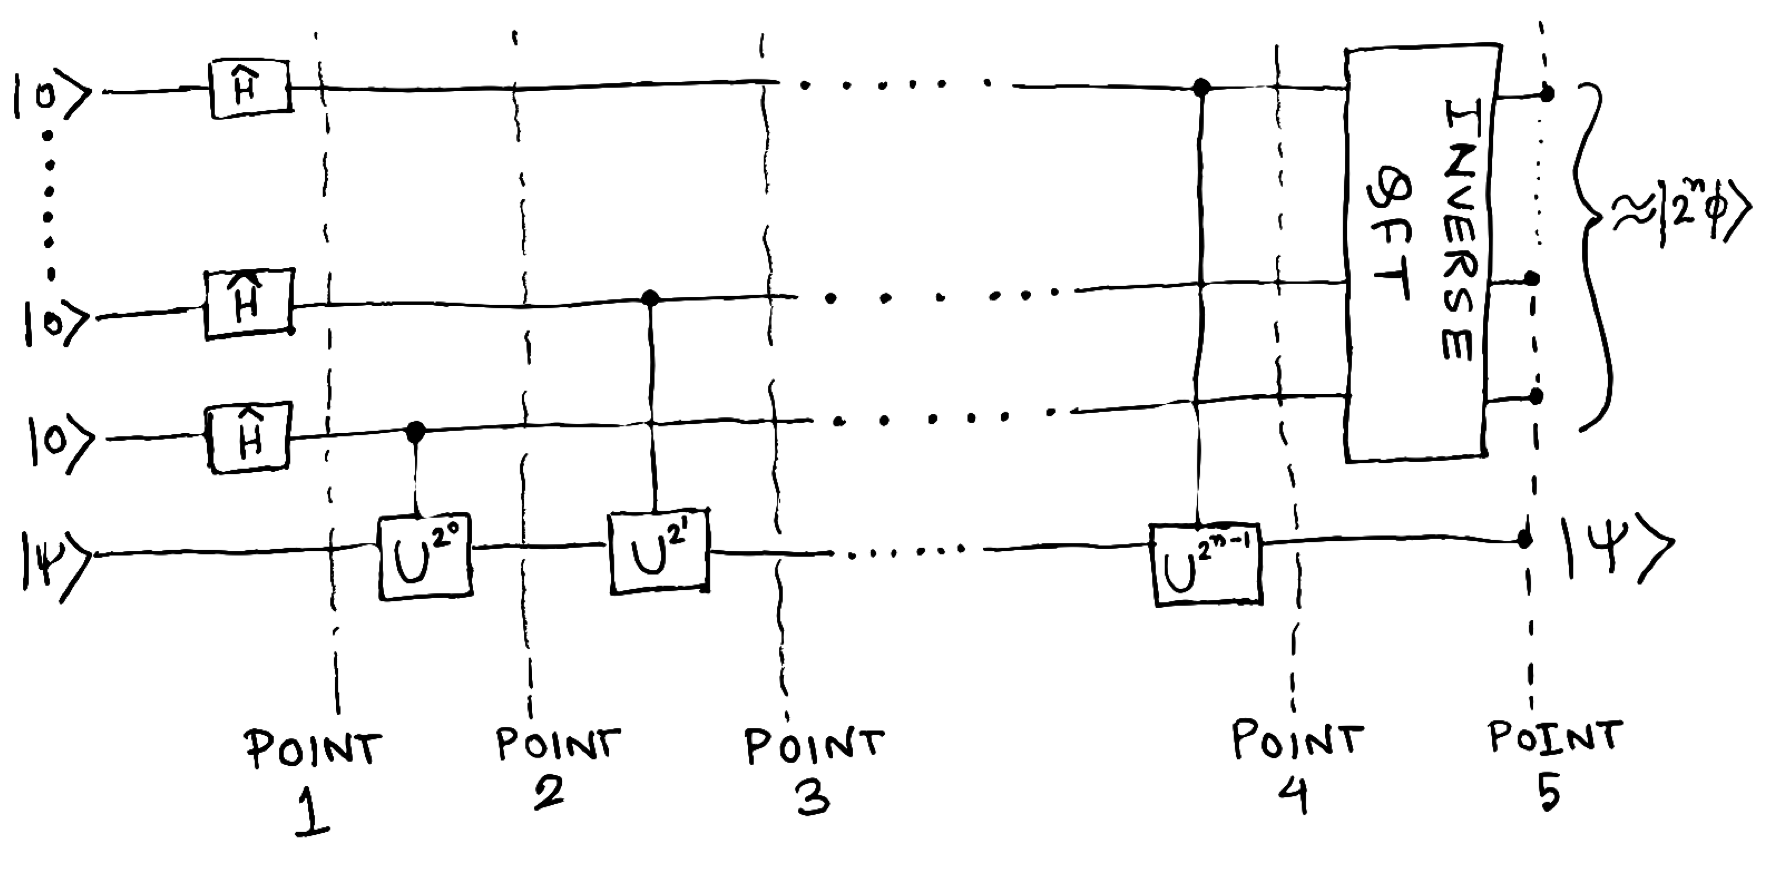
\includegraphics[width=0.99\textwidth]{QPE.png}
    \caption{Circuit for performing quantum phase estimation}
    \label{QPE_circuit}
\end{figure}

Now let us look at the circuit in Fig.~\ref{QPE_circuit}. We prepare the control register, consisting of $n$ qubits, with each qubit initially in state $\ket{0}$. The state $\ket{\Psi}$ is fed into the target register.

\begin{enumerate}
    \item Then, at point 1, each control qubit (with index ranging from $n-1$, which is the topmost control qubit, to 0, which is the bottommost control qubit) is in $\frac{1}{\sqrt{2}}\left(\ket{0}+\ket{1}\right)$ and the state of the entire system is
    \begin{align*}
        \ket{\Phi_1}&{}=\left[\otimes_{l=n-1}^{0}\frac{1}{\sqrt{2}}\left(\ket{0}+\ket{1}\right)\right]\otimes\ket{\Psi}\\
        &{}=\left[\frac{1}{\sqrt{2^n}}\sum_{j=0}^{2^n-1}\ket{j}\right]\otimes\ket{\Psi},
    \end{align*}
    where $\ket{j}$ denotes the $j$-th computational basis
    \item Next a controlled-$\hat{U}^{2^0}$ gate is operated on the target state $\ket{\Psi}$ with the $0$-th qubit of the control register acting as the control qubit. In accordance with Eq.~\ref{representativeCROT}, the resulting state at point 2 is
    \begin{align*}
        \ket{\Phi_2}=\left[\otimes_{l=n-1}^{1}\frac{1}{\sqrt{2}}\left(\ket{0}+\ket{1}\right)\right] \otimes \frac{1}{\sqrt{2}}\left(\ket{0}+\left(e^{2^0 . 2\pi i \phi}\right)\ket{1}\right) \otimes \ket{\Psi}
    \end{align*}
    \item Similarly, the state at point 3 is
    \begin{align*}
        \ket{\Phi_3}=\left[\otimes_{l=n-1}^{2}\frac{1}{\sqrt{2}}\left(\ket{0}+\ket{1}\right)\right] \otimes \frac{1}{\sqrt{2}}\left(\ket{0}+\left(e^{2^1 . 2\pi i \phi}\right)\ket{1}\right) \otimes \frac{1}{\sqrt{2}}\left(\ket{0}+\left(e^{2^0 . 2\pi i \phi}\right)\ket{1}\right) \otimes \ket{\Psi}
    \end{align*}
    \item Ultimately, at point 4, the state of the system becomes
    \begin{align*}\label{QPE_4}
        \ket{\Phi_4}&{}= \frac{1}{\sqrt{2^n}}\left(\ket{0}+e^{2\pi i 2^{n-1}\phi}\ket{1}\right)\otimes\hdots\otimes \left(\ket{0}+e^{2\pi i 2^0\phi}\ket{1}\right)\otimes \ket{\Psi}\\
        &{}= \left[\frac{1}{\sqrt{2^n}} \sum_{j=0}^{2^n-1}e^{2\pi i j \phi}\ket{j}\right]\ket{\Psi}\numberthis
    \end{align*}
    If, for some integer $k<2^n$, we have $\phi=\frac{k}{2^n}$, then from Eq.~\ref{QFT_2}, the term inside the square brackets can be seen to be $\hat{U}_{\mathrm{QFT}}\ket{k}$.
    \item Thus, if $\phi=\frac{k}{2^n}$, then an inverse QFT of the $n$ control qubits will produce, at point 5, the computational basis vector $\ket{k}=\ket{2^n\phi}$ will full certainty. This will conclude the process of finding the eigenvalue of $\ket{\Psi}$. The target register stays at state $\ket{\Psi}$.

    \begin{align}
        \ket{\Phi_5}=\ket{2^n\phi}\otimes\ket{\Psi}
    \end{align}
    
    If $\phi \neq \frac{k}{2^n}$ for any integer $k<2^n$, then the inverse QFT of the  quantity inside the square brackets in Eq.~\ref{QPE_4} will not be a computational basis vector, but rather a linear combination thereof. Thus, upon measurement, the control register will collapse, with high probability, to the computational basis vector corresponding to the closest integral approximation of $2^n\phi$.
\end{enumerate}

This does not seem to be very helpful in this particular form. After all, if the goal is to find an eigenvalue $\phi$ of $\hat{O}$, we will probably not know the corresponding eigenvector $\ket{\Psi}$ in the first place. Let us see what happens if, instead of the eigenstate $\ket{\Psi}$, we insert a generic state
\begin{align}
    \ket{V}=\sum_p \alpha_p\ket{\Psi_p}
\end{align}
in the target register such that
\begin{align}
    \hat{O}\ket{\Psi_p}=\phi_p\ket{\Psi_p}.
\end{align}
Note that if $\hat{O}$ is associated with any observable, then it is Hermitian and therefore, any generic state can be expressed as a linear combination of its eigenstates.
\begin{enumerate}
    \item Now, at point 1, we have
    \begin{align*}
        \ket{\Phi_1}=\sum_p \alpha_p \left[\frac{1}{\sqrt{2^n}}\sum_{j=0}^{2^n-1}\ket{j}\right]\otimes\ket{\Psi_p}
    \end{align*}
    \item At point 4, the state would be
    \begin{align*}
        \ket{\Phi_4} &{} =\sum_p \alpha_p \left[\frac{1}{\sqrt{2^n}} \sum_{j=0}^{2^n-1}e^{2\pi i j \phi_p}\ket{j}\right]\otimes\ket{\Psi_p}\\
        &{} = \alpha_1 \left[\left(\frac{1}{\sqrt{2^n}} \sum_{j=0}^{2^n-1}e^{2\pi i j \phi_1}\ket{j}\right)\otimes\ket{\Psi_1}\right] + \alpha_2 \left[\left(\frac{1}{\sqrt{2^n}} \sum_{j=0}^{2^n-1}e^{2\pi i j \phi_2}\ket{j}\right)\otimes\ket{\Psi_2}\right] + \hdots
    \end{align*}
    %What happens now if we do an inverse Fourier transform of the control register alone? 
    This expression indicates that, if, for some integer $k<2^n$, we have $\phi_p=\frac{k}{2^n}$, then an inverse Fourier transform of the control register will produce the computational basis vector $\ket{2^n\phi_p}$ with a probability of $|\alpha_p|^2$.
\end{enumerate}
\end{document}
